\subsection{Implementering af database}

Til implementering af databasen samt kommunnikation med denne benyttes programmet XAMPP. Programmet opretter en lokal apache webserver samt database på en given computer, der fungerer som et Localhost miljø. Den lokale webserver simulerer dertil en ekstern webserver, hvilket giver et passende miljø til udvikling og test af app'en. Databasen er udarbejdet i phpMyAdmin, der er et online databaseadministrationssystem og understøtter Structured Query Language (SQL) \autoref{silbershatz2011}. 
Databasen er implementeret under navnet \textit{$db_KOL$} og indeholder fire tabeller \textit{users}, \textit{kondi}, \textit{beloenninger} og \textit{vennerelation}. Hertil er værdityperne oprettet som beskrevet i \autoref{ERdiagram}.

Kommunikation mellem Android Studio og databasen kan ikke forekomme direkte, hvorfor PHP: Hypertext preprocessor scripts benyttes. PHP er et Server-Side Scripting Language, hvilket køres på serveren og muliggører systemet kan tilgå databasen \autoref{silbershatz2011}. 
Der er oprettet et php-script, \textit{config}, der indeholder informationerne host, bruger, adgangskode samt navn på den oprettede database. Dette script inkluderes i et seperat script, \textit{$DB_connect$}, til at etablerer forbindelsen til databasen. Der er ligeledes opstillet et PHP-scripts, der manupulerer data i databasen ved hjælp SQL-kommandorer. Disse SQL kommandorer manupulerer i forhold til information fået fra app'en. 

Informationen sendes fra app'en som en Java Script Object Notation (JSON) repræsentation. JSON er et dataoverførselsformat, der  gør det muligt at pakke data som et object eller array. PHP-scripts tjekker, hvorvidt der bliver sendt en værdi i det respektive navn. Er værdierne sat og ikke NULL, ligges værdierne i en ny variabel. Et eksempel af dette ses af \autoref{fig:phplogind}, hvor et udklip af PHP-scriptet for log ind er visualiseret. 

\begin{figure} [H]
\centering
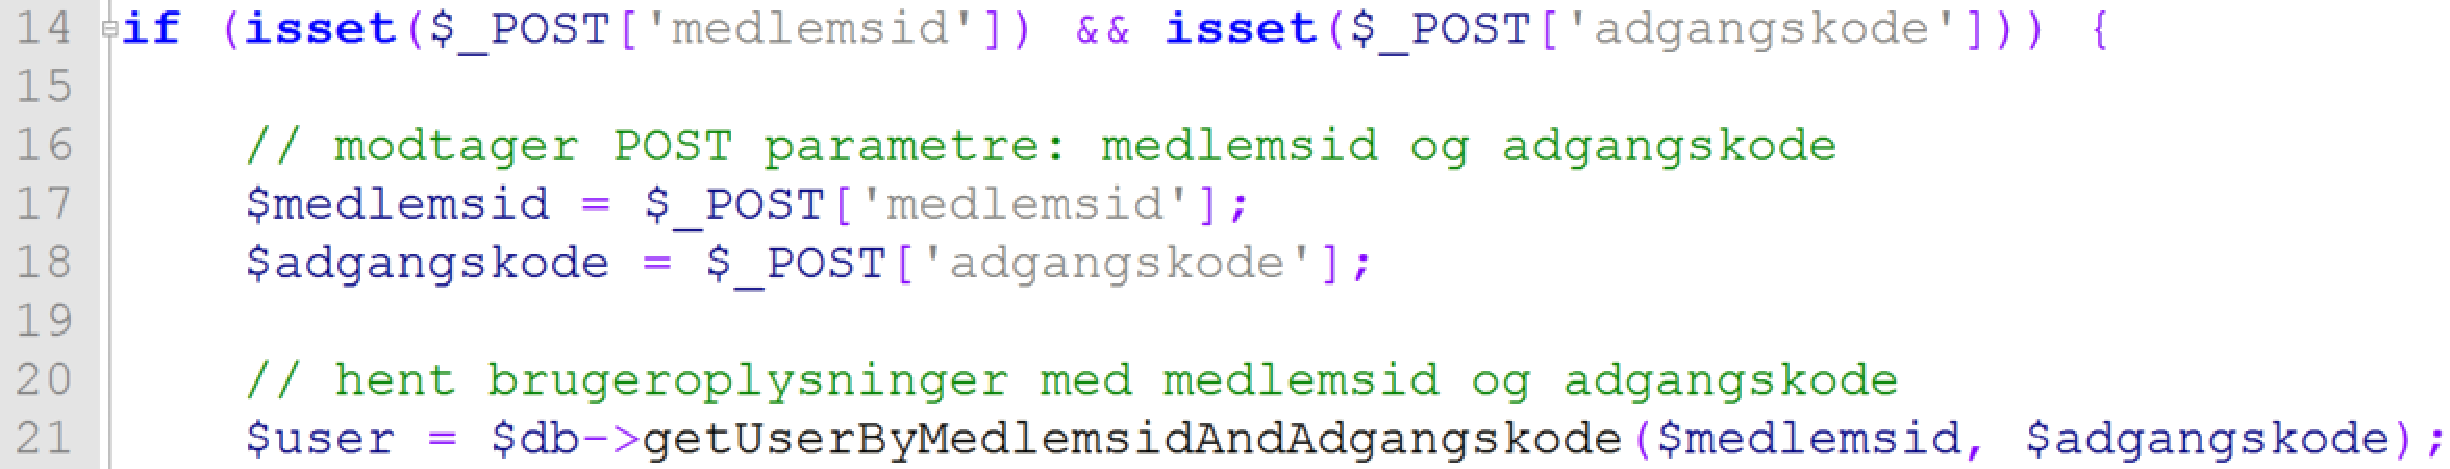
\includegraphics[width=1\textwidth]{figures/imple/phplogind}
\caption{Udklip af log ind PHP-script, hvor medlemsid samt adgangskode modtages og indsættes i tilhørende variabler, der benyttes i et funktionskald.}
\label{fig:phplogind}
\end{figure}

\noindent
Dette udklip viser, hvordan koden modtages og gemmes i nye variabler. Værdierne gemmes i et associativt array, der ved hjælp af en POST-metode gør det muligt at overføre data'en til et andet script, \textit{$db_functions$}, hvori SQL-kommandoen udføres. Linje 21 viser, hvordan variablerne benyttes i et funktionskald, der eksekveres i \textit{$db_functitons$}. Denne funktion er illustreret af \autoref{fig:phplogindsql}.

\begin{figure} [H]
\centering
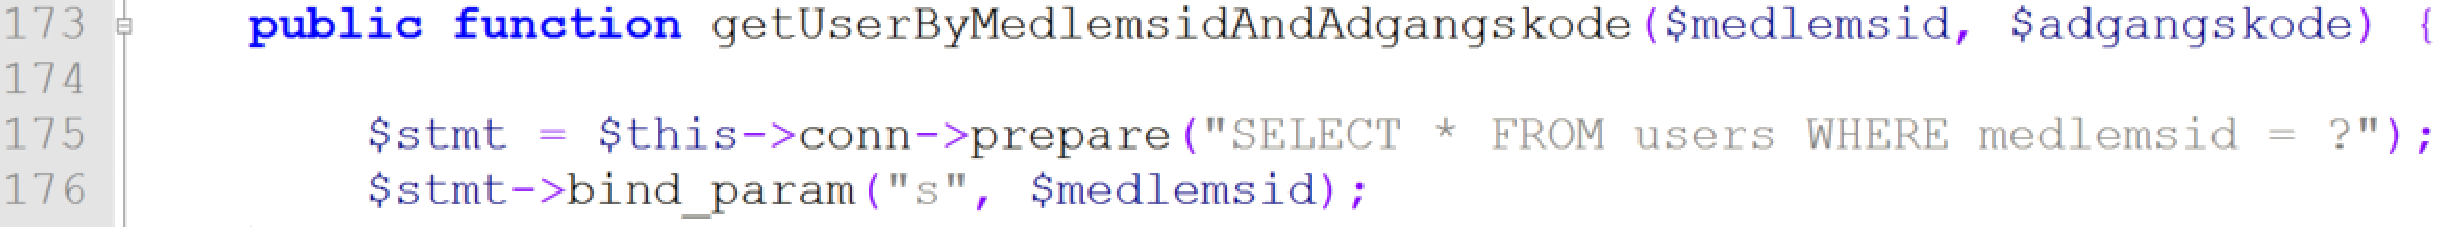
\includegraphics[width=1\textwidth]{figures/imple/phplogindsql}
\caption{SQL-kommando for funktionen log ind.}
\label{fig:phplogindsql}
\end{figure}

\noindent
Det ses af \autoref{fig:phplogindsql}, hvordan en SQL-kommando udføres. Denne SQL-kommando henter alt fra tabellen \textit{users} tilhørende medlemsid i databasen, der er lig spørgsmåltegn. Spørgsmåltegnet markerer et bindingspunkt, hvorpå en parametre kan tilknyttes. Parametren, der bindes på, fremgår af linje 176, hvoraf \textit{"s"} indikerer, at medlemsid'et er af typen string. I dette tilfælde valideres log ind informationerne førend user returneres til log ind PHP-scriptet, der håndterer user, hvilket fremgår af \autoref{fig:phplogindresp}.


\begin{figure} [H]
\centering
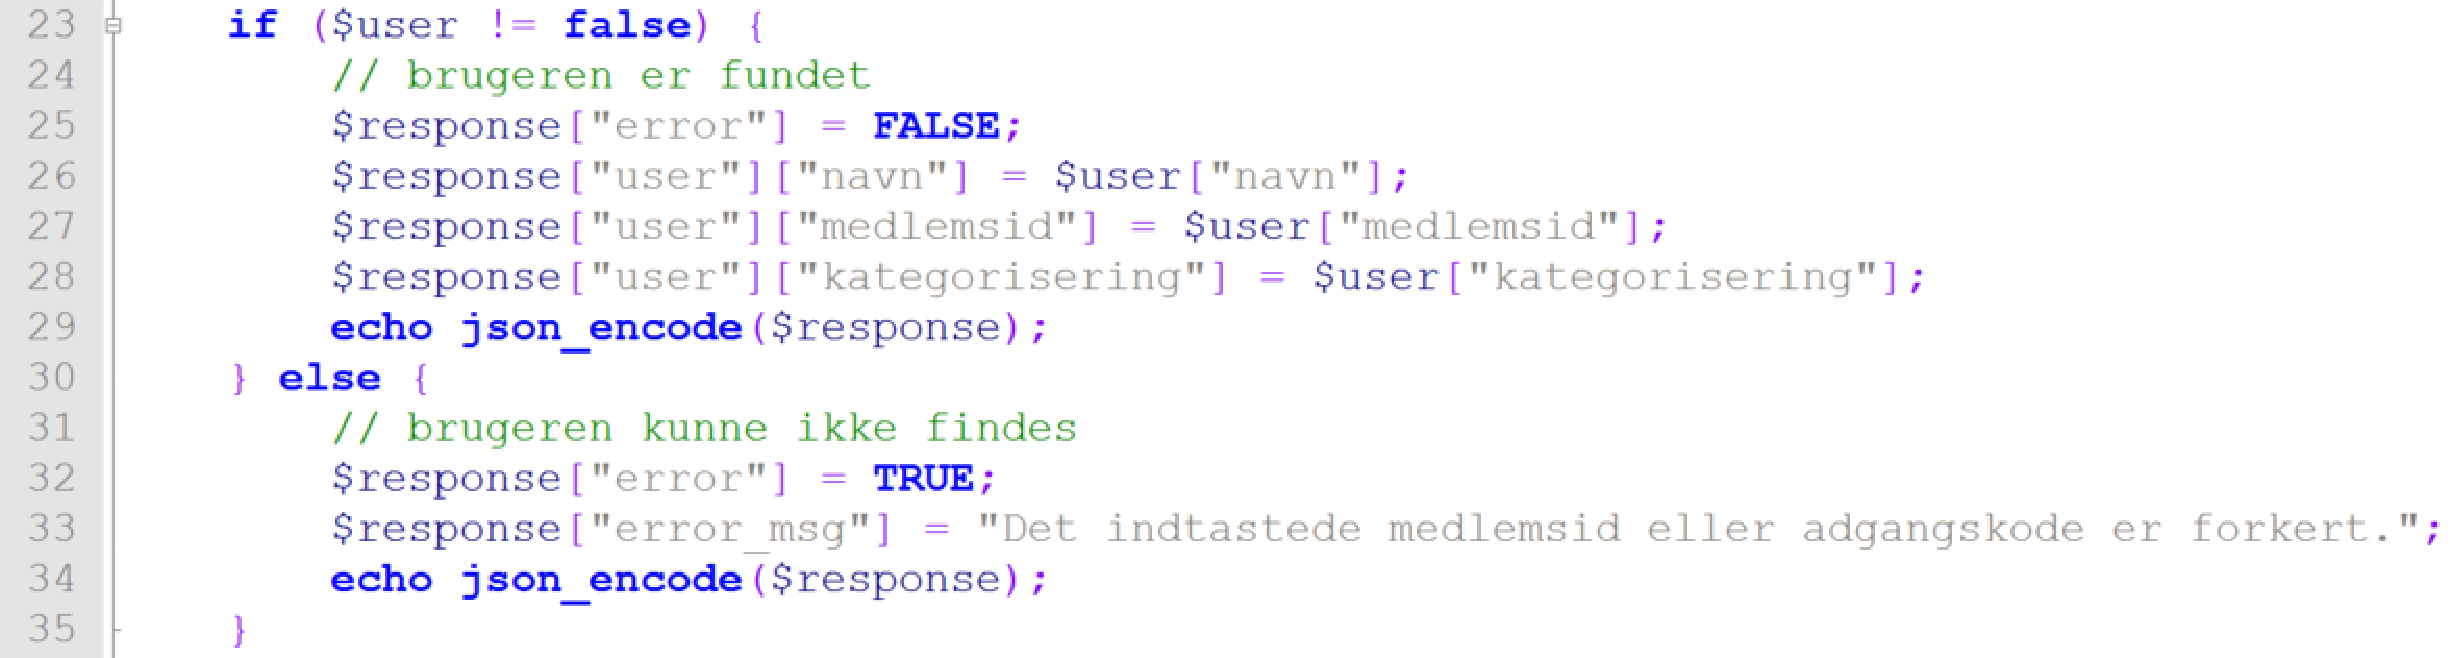
\includegraphics[width=1\textwidth]{figures/imple/phplogindresp}
\caption{Datahåndtering i PHP-scriptet førend respons til app'en.}
\label{fig:phplogindresp}
\end{figure}


\noindent
Som det ses af \autoref{fig:phplogindresp} opstilles if/else statement, der håndterer, hvorvidt user returneres. Hvis user returneres bliver brugerdata gemt i \textit{response}, der sendes tilbage til app'en som en JSON repræsentation. Returneres user ikke, gemmes en fejlmeddelelse i \textit{response}, der ligeledes sendes til app'en som en JSON repræsentation. 
Der er i javakoden opsat en \textit{Response.listener}, der lytter efter respons. Ved respons oprettes et nyt JSON objekt, hvori responset lagres, således dette kan benyttes i app'en. 






For at indikere, hvilket script systemet skal tilgå opstilles URL links, der definerer ip-adressen på serveren samt placeringen af det ønskede script.

